\documentclass[../tesis_main.text]{subfiles}



\chapter{Detección de objetos}
En este capítulo se aborda el desarrollo de los algoritmos para la detección y extracción de características de objetos propuestos en los objetivos de este trabajo. La metodología de desarrollo de este capítulo se divide en las tareas descritas a continuación:\\

	\begin{itemize}
		\item{Segmentación de planos}
		\item{Extracción de planos}
		\item{Segmentación de objetos}
		\item{Cálculo del centroide de un objeto}
		\item{Estimación a la orientación de un objeto}
	\end{itemize}

	Es importante mencionar que los desarrollos reportados en este trabajo fueron realizados en la plataforma para el desarrollo de software para robots ROS (Robot Operative System por sus siglas en inglés)\cite{quigley2009ros}, alojado en el sistema operativo Ubuntu 16.04. (Ver sección 5)\\

	%**Acondicionamiento de Nube de puntos(???) Transformaciones(???)

	\section{Segmentación de planos con RANSAC}

		Para el desarrollo del algoritmo RANSAC se utilizó el sensor Kinect dado que este sensor, además de una imagen de color, proporciona información sobre la profundidad de los objetos. Con un manejo adecuado de ambos datos se pueden conseguir avances notables en el campo de la visión computacional. Para el desarrollo del algoritmo se hizo uso de la información de profundidad de los objetos.\\

		\begin{figure}[h!]
			\begin{center}
			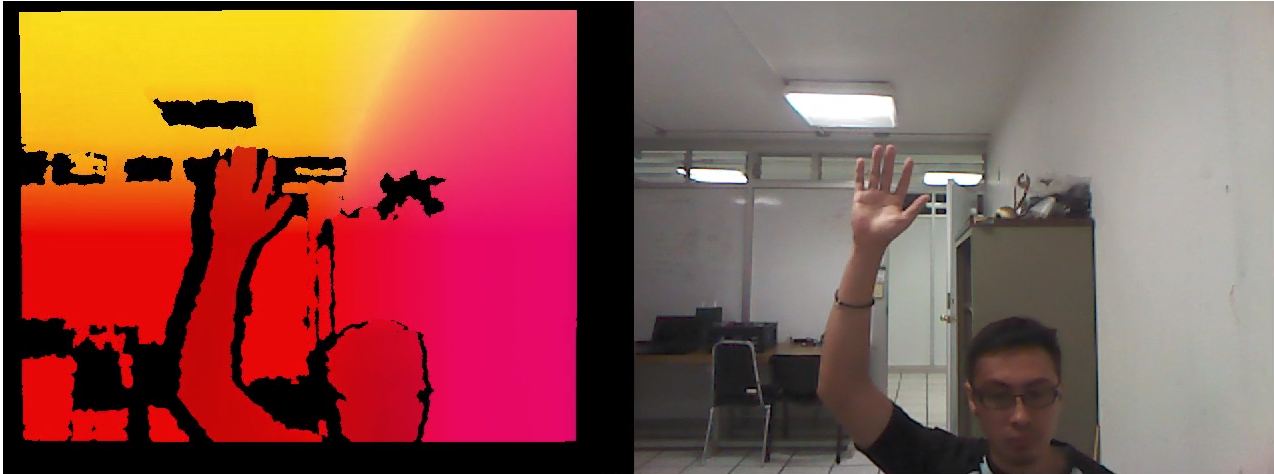
\includegraphics[width=12.0cm, height=4.5cm]{vision/pointCloud1.png}	
			\caption{Imagen típica de la información otorgada por el sensor Kinect.}
			\end{center}
		\end{figure}
		
		Se desarrolló un programa en lenguaje C++ para segmentar los planos. La información de profundidad entregada por el Kinect, se da en una matriz donde cada elemento $i, j$ contiene la información de profundidad obtenida por el sensor, como se explica a continuación.\\


		Cada elemento de la matriz contiene información de un punto $p = (x, y, z)$ donde el haz infrarojo fue reflejado, esto nos permite conocer la distancia a la cual se encuentra un objeto, o su superficie. La información que nos entrega el sensor en forma de matriz es de dimensiones 640X480 por tanto consta de 307,200 elementos en total.  Dentro de este conjunto de datos se buscan las superficies planas.\\

		Se programó el algoritmo RANSAC para extraer planos en C++, el código se puede consultar en la página \cite{githubTesis}.\\

		Para la correcta implementación del algoritmo fue necesario tomar algunas consideraciones, por ejemplo: descartar del procesamiento todos aquellos píxeles que no proporcionen información relevante de profundidad para reducir el tiempo de procesamiento del algoritmo.\\

		Para la construcción de planos se tomaron tres puntos aleatorios y se construyeron dos vectores a partir de los puntos y se realizó el producto cruz entre estos.\\ 

		\begin{equation}
		\begin{split}
			p_1 = rnd (datos) \cr
			p_2 = rnd (datos) \cr
			p_3 = rnd (datos) \cr
			\vec{v_1} = p_1 - p_2 \cr
			\vec{v_2} = p_1 - p_3 \cr
			\vec{N} = \vec{v_1} \times \vec{v_2} \cr
		\end{split}
		\end{equation}

		Conocemos la ecuación general del plano:\\

		\begin{equation}
			\begin{split}
			\Pi: Ax + By + Cz + D = 0
			\end{split}
		\end{equation}


		donde: A, B, C son las componentes del vector normal respectivamente y D la podemos calcular como:\\

		\begin{equation}
			\begin{split}
			D = -(A p_{1_{x}} + Bp_{1_{y}} + Cp_{1_{z}})
			\end{split}
		\end{equation}


		Por lo tanto con tres puntos seleccionados aleatoriamente tenemos un modelo de plano generado aleatoriamente, lo cual es el primer requerimiento para el algoritmo.\\ 

		Posteriormente se comparó el resto de la información con ese modelo propuesto aleatoriamente y verificamos que tan buen modelo es. Para ello calculamos la distancia euclidiana de cada punto al plano propuesto, si la distancia es menor que cierto umbral lo consideramos como parte del modelo e incrementamos el numero de valores típicos que empatan con el modelo (``inliers").\\

		Del mismo modo se buscaba que el numero de valores típicos que empataran con el modelo fuera al menos el 60\% del total de datos. De otro modo la implementación a nivel de algoritmo devolvía un modelo vacío. En apartado correspondiente a los resultados se trata este tema con mayor profundidad.\\


		\begin{figure}[h!]
			\begin{subfigure}[t]{.5\textwidth}
			\centering
			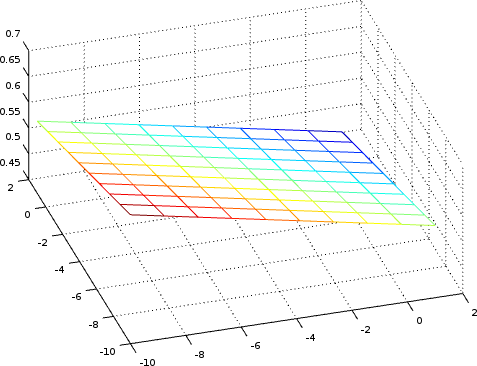
\includegraphics[width=5.5cm, height=3.5cm]{planes/plane.png}	
			\caption{Grafico de un plano en tercera dimensión.}
			\end{subfigure}%
			\begin{subfigure}[t]{.5\textwidth}
			\centering
			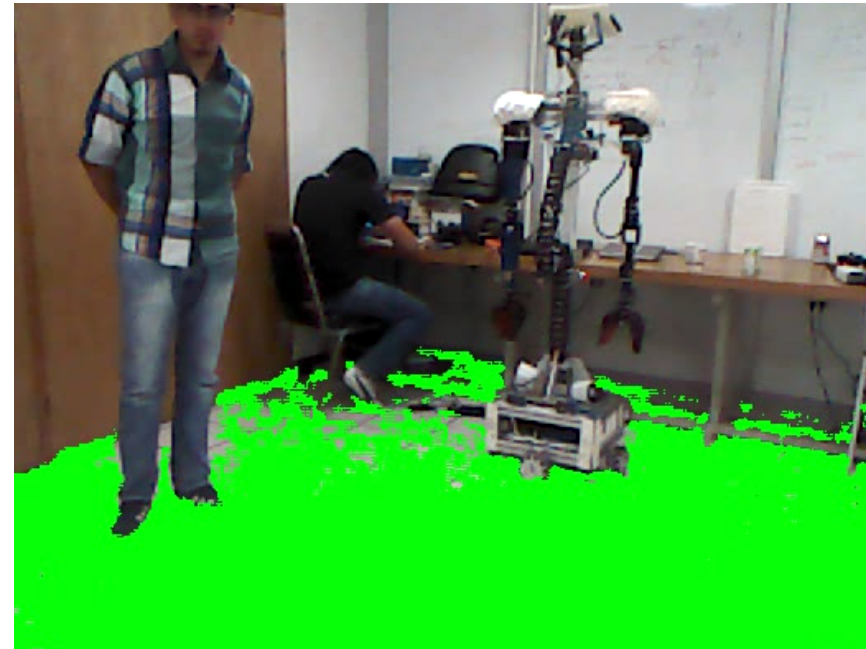
\includegraphics[width=6.5cm, height=3.5cm]{planes/planeSegmentation5.png}
			\caption{Segmentación de un plano utilizando el algoritmo RANSAC con un número de iteraciones igual a 70 y un umbral de 2 cm (Plano en color verde). }
			\end{subfigure}

			\caption{Planos y su representación en 3D.}
		\end{figure}


		Por ahora el algoritmo no restringe su búsqueda a planos horizontales o verticales, queda como trabajo futuro el desarrollo de una búsqueda selectiva de planos con características similares a una mesa, destacando características de horizontalidad y altura.\\


	\section{Extracción de objetos}
		
		Una vez  que se encontró la nube de puntos perteneciente al plano, se prosiguió a ubicar espacialmente los objetos que se encontraban sobre el plano. Se realizó la extracción de objetos con las siguientes restricciones:\\

		\IncMargin{1em}
		\begin{algorithm}[H]
		\SetKwData{Left}{left}\SetKwData{This}{this}\SetKwData{Up}{up}
		\SetKwFunction{Union}{Union}\SetKwFunction{FindCompress}{FindCompress}
		\SetKwInOut{Input}{input}\SetKwInOut{Output}{output}
		
		\Input{Nude de puntos organizada}
		\Input{Modelo del plano}
		\BlankLine
		
		Sea:
		\textbf{Condiciones iniciales}\;
		$p \leftarrow$ Conjunto total de puntos obtenidos del sensor\;
		$p_{\pi} \leftarrow$ Conjunto de puntos pertenencientes al modelo del plano\;
		$p_0 \leftarrow$ Conjunto de puntos pertenencientes a un objeto\;
		$p_{extra} \leftarrow$ Conjunto de puntos con restricciones adicionales \;
		\BlankLine
		\BlankLine

		$p \leftarrow \{ p_1, p_2, p_3... p_n \}$\;
		$p_{\pi} \leftarrow \{ p_{\pi_{1}}, p_{\pi_{2}}, p_{\pi_{3}}... p_{\pi_{n}} \}$\;
		$p_0 \leftarrow  \{ \emptyset \}$\;
		$p_{extra} \leftarrow \{ (x, y, x,) : x < 0.5[m], z < p.z \forall p \in p_{\pi} \}$ \;

		\BlankLine
		\BlankLine
		\BlankLine

		$p_0 = p - p_{\pi} - p_{extra}$\; 
		
		\BlankLine
		\BlankLine
		\BlankLine

		\textbf{return} $p_0$ \;
		\caption{Algoritmo para extracción de objetos de una nube de puntos organizada.}
		\label{objExtract_algorithm}
		\end{algorithm}\DecMargin{1em}


		De otro modo esto sería igual a:\\

		\begin{itemize}
			\item{Supresión de los puntos pertenecientes al plano.}
			\item{Supresión de los puntos por debajo del plano.}
			\item{Supresión de los puntos más allá de 50[cm] respecto al punto más cercano en x.}
		\end{itemize}

		\begin{figure}

			\begin{subfigure}[h]{.5\textwidth}
			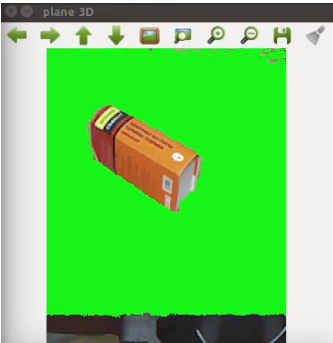
\includegraphics[width=5.5cm, height=4.0cm]{objs/object1.png}	
			\caption{Extracción de los puntos que pertenecen al objeto.}
			\end{subfigure}%
			\begin{subfigure}[h]{.5\textwidth}
			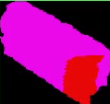
\includegraphics[width=4.5cm, height=3.5cm]{objs/object1_pc.png}
			\caption{Información de profundidad del objeto.}
			\end{subfigure}
			\label{Fig:objExtra}
			\caption{Extracción de información del objeto.}
		\end{figure}

		Posterior a este proceso tenemos como resultado un conjunto de puntos reflejados sobre un objeto sólido con las distancias proyectadas sobre los tres ejes coordenados respecto del robot.\\


	\section{Aproximación de orientación de objetos con PCA}

		El análisis de componentes principales se usa abundantemente en muchas formas de análisis de datos. En este caso se utilizará como una metodología para reducir un conjunto de datos a una dimensión inferior. Más concretamente la forma en que podemos obtener una base ortogonal del conjunto de datos, que represente la distribución de los puntos proyectados sobre el objeto. Esta base, representará la dirección de la distribución de los puntos del objeto, y por tanto encontraremos la dirección del objeto mismo respecto al robot.\\  

		\subsection{Adquisición de datos y cálculo de la media}
			La adquisición de datos se realizó mediante la extracción de los puntos pertenecientes al objeto. Cada uno de los datos perteneciente al conjunto de puntos posee tres características:\\

			\begin{itemize}
				\item{La distancia al objeto  proyectada sobre el eje $x$}
				\item{La distancia al objeto  proyectada sobre el eje $y$}
				\item{La distancia al objeto  proyectada sobre el eje $z$}
			\end{itemize} 

			Por lo tanto, de una nube de puntos como la mostrada en la figura \cite{Fig:objExtra} podemos extraer medidas de dispersión, y medidas de tendencia central. Se partió con el cálculo de la media de los datos. $\bar{X}, \bar{Y}, \bar{Z}.$ El punto $P(\bar{X}, \bar{Y}, \bar{X})$ representa el centroide del objeto. Conociendo este punto podemos conocer la ubicación espacial del objeto respecto del robot y determinar si es manipulable (si se encuentra dentro del área de trabajo) y conocer las coordenadas a donde debemos llevar el efector final del manipulador.\\

			Aunque el cálculo del centroide del objeto es operacionalmente simple este resultado puede no representar correctamente el centroide real del objeto. La extracción de la informacion del objeto está sujeta a la perpectiva de la cámara con respecto del objeto en cuestión. De esta manera si la posición de la cámara con respecto del objeto se aproxima a una vista lateral se reducirá la cantidad de hazes de luz proyectada sobre la superficie del objeto. En la figura \cite{Fig:objCentroide} se lográ a apreciar que el punto representante del controide no coincide con con el centroide real de los objetos.\\

		% 	Para realizar el cálculo de la media se cuantifico el número de puntos pertenecientes al objeto, $(n)$. Posteriormente, para todos los puntos pertenecientes al conjunto $n$ se sumaron sus valores en $\bar{X}, \bar{Y}, \bar{Z}$, respectivamente. Y posteriormente se dividieron entre $n$.\\

		% \IncMargin{1em}
		% \begin{algorithm}[H]
		% \SetKwData{Left}{left}\SetKwData{This}{this}\SetKwData{Up}{up}
		% \SetKwFunction{Union}{Union}\SetKwFunction{FindCompress}{FindCompress}
		% \SetKwInOut{Input}{input}\SetKwInOut{Output}{output}
		
		% \Input{Nude de puntos organizada perteneciente al objeto segmentado}
		% \Output{$ \bar{X},  \bar{Y}, \bar{Z}$}
		% \BlankLine
	
		% $Inicializaci\acute{o}n$ de $variables$\;
		% $\bar{X} = 0$\;
		% $\bar{Y} = 0$\;
		% $\bar{Z} = 0$\;
		% \BlankLine
		% \BlankLine
	

	 %    \For{ cada punto \textbf{in} datos(objeto)}
		% {
		% 	$X_{total} = X_{total} + dato_{x}$\;
		% 	$Y_{total} = Y_{total} + dato_{y}$\;
		% 	$Z_{total} = Z_{total} + dato_{z}$\;
		% }
		% \BlankLine
		
		% $\bar{X} = \dfrac{X_{total} } {n} $\;
		% $\bar{Y} = \dfrac{Y_{total} } {n} $\;
		% $\bar{Z} = \dfrac{Z_{total} } {n} $\;
		% \BlankLine
		% \BlankLine

		% \textbf{return} $P(\bar{X}, \bar{Y}, \bar{Z})$\;
		% \caption{Cálculo del centroide de un objeto basado en nubes de puntos}
		% \label{centroide}
		% \end{algorithm}\DecMargin{1em}


		%%Ïmagen centroides Rviz.
		\begin{figure}[h!]
			\begin{subfigure}[h]{.5\textwidth}
			\centering
			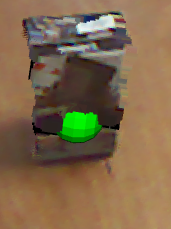
\includegraphics[width=3.5cm, height=5.0cm]{objs/centroid3.png}	
			\end{subfigure}%
			\begin{subfigure}[h]{.5\textwidth}
			\centering
			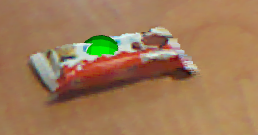
\includegraphics[width=6.0cm, height=3.5cm]{objs/centroid5.png}
			\end{subfigure}
		\caption{Segmentación de un objeto y su correspondiente centroide (punto verde).}
		\label{Fig:objCentroide}
		\end{figure}
			

		\subsection{Cálculo de la matriz de covarianza}
			Dada una variable estadística n-dimensional  $(X_1, X2,X3,...,Xn)$, llamaremos matriz de covarianzas a la matriz cuadrada, $n \times n$, que disponga en su diagonal principal de las varianzas de cada una de las distribuciones marginales unidimensionales, y en los elementos no-diagonales $(i,j)$ de las correspondientes covarianzas entre cada dos variables $S_{ij}.$\\

			Para ello se hizo uso de las expresiones matemáticas correspondientes:\\

			 \begin{equation}
				\begin{split}
					var(X) = \dfrac{\Sigma^n_{i=1} (X_i - \bar{X} ) (X_i - \bar{X}) } { n }
				\end{split}
			\end{equation}

			\begin{equation}
			\begin{split}
				cov(X, Y) = \dfrac{\Sigma^n_{i=1} (X_i - \bar{X} ) (Y_i - \bar{Y}) } { n }
			\end{split}
			\end{equation}

			A continuación se anexa en código correspondiente al cálculo de las varianzas y covarianzas.\\



			\begin{lstlisting}[language=c++, caption=Cálculo de varianzas y covarianzas]
//Calculate covariance matrix
for(int j = 0; j < object.rows; j++)
	for (int i = 0; i < object.cols; i++)
	{
		px = object.at<cv::Point3f>(j,i);
		if ( px != cv::Point3f(0.0, 0.0, 0.0) && px != cv::Point3f(0, 255, 0))
		{
			var_x += pow( (px.x - centroid[0]), 2 );
			var_y += pow( (px.y - centroid[1]), 2 );
			var_z += pow( (px.z - centroid[2]), 2 );
			cov_xy += ( px.x - centroid[0] )*( px.y - centroid[1] );
			cov_xz += ( px.x - centroid[0] )*( px.z - centroid[2] );
			cov_yz += ( px.y - centroid[1] )*( px.z - centroid[2] );
			n++;
		}
	}

var_x /= n;
var_y /= n;
var_z /= n;

cov_xy /= n;
cov_xz /= n;
cov_yz /= n;

cov_matrix << var_x,  cov_xy, cov_xz,
				 cov_xy,  var_y, cov_yz,
				 cov_xz, cov_yz,  var_z;
			\end{lstlisting}

			Posteriormente se propuso a encontrar los valores de los vectores propios asociados a la matriz de covarianzas. En la literatura existen múltiples métodos numéricos para la solución de esta problemática, como la puesta a prueba de dichos algoritmos no es el propósito de este trabajo se optó por utilizar la librería \textbf{eigen}. Por tanto, una vez construida la matriz de covarianzas M, se utiliza la instrucción:\\

			\begin{lstlisting}[language=c++, caption=Cálculo de varianzas y covarianzas]
Eigen::SelfAdjointEigenSolver<Eigen::MatrixXf> eig(cov_matrix); \end{lstlisting}

			La instrucción \textit{Eigen::SelfAdjointEigenSolver$<$Eigen::MatrixXf$>$} nos devuelve un objeto \textit{eig} cuyos atributos son \textit{eigenvalues()} y \textit{eigenvectors()}. Con ayuda de esta librería podemos obtener fácilmente los vectores propios de la matriz M. Es importante mencionar que el atributo \textit{eigenvectors()} del objeto \textit{eig} se encuentra normalizado; por lo tanto es conveniente darle un escalamiento relacionado con la dispersión de los datos. De este modo se optó por multiplicar cada uno de los vectores propios por su correspondiente valor de desviación estándar.\\

			\begin{figure}[ht!]

				\begin{subfigure}[h]{.5\textwidth}
				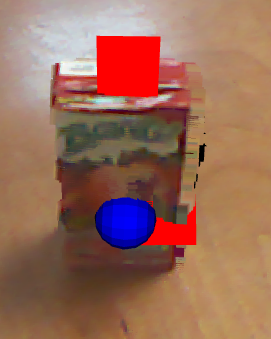
\includegraphics[width=3.5cm, height=5.0cm]{objs/centroid_1.png}	
				\end{subfigure}%
				\begin{subfigure}[h]{.5\textwidth}
				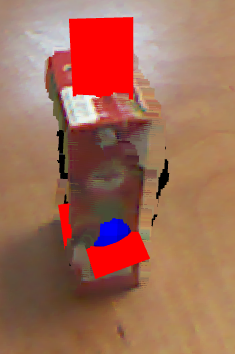
\includegraphics[width=3.5cm, height=5.0cm]{objs/centroid2.png}
				\end{subfigure}
			
			\caption{Segmentación de un objeto y sus correspondientes ejes principales (rojo).}

			\end{figure}



	\subsection{Cálculo de rotación del objeto}
	Una vez que se obtivieron los eigenvectores de la matriz de covarianzas estos indican las direcciones en los cuales tiene una mayor distribución la nube de puntos del objeto en cuestión. Por la naturaleza de los eigen-vectores y al tratarse de un espacio tridimensional, estos ejes forman un sistema ortogonal; por lo tanto son perpendiculares entre sí.\\

	Por tal motivo basta con conocer los cosenos directores de cada uno de los eigenvetores con el eje coordinado del robot, comparalos en mágnitud y determinar los ángulos roll, pitch y yaw del objeto con respecto del robot.\\

	%**** Eigenvectores\\

	\subsubsection{Componentes y cosenos directores de un vetor.}

	Se llama componentes de un vector $\vec{A}$ respecto del sistema de coordenadas con oriegen O y ejes \textit{x, y} a las proyecciones de $\vec{A}$ sobre los ejes, sea dicho de otro modo, los números:\\

	\begin{equation}
	\begin{split}
		a_1 = x_2 - x_1 \cr 
		a_2 = y_2 - y_1 \cr
	\end{split}
	\end{equation}


	Transaladando esta idea a un espacio tridimensional los componentes de un vector están determinados por la forma:\\

	\begin{equation}
	\begin{split}
		a_1 = x_2 - x_1 \cr
		a_2 = y_2 - y_1 \cr
		a_3 = z_2 - z_1 \cr
	\end{split}
	\end{equation}


	\begin{figure}[H]
		\centering
		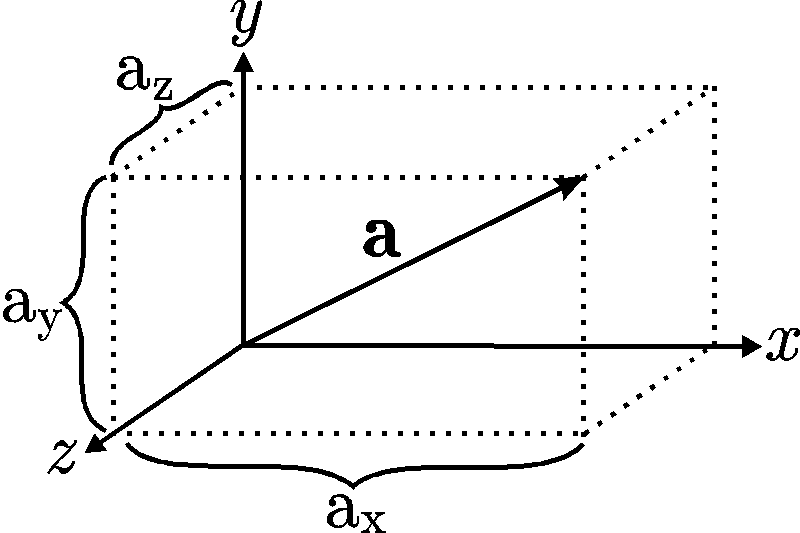
\includegraphics[width=8.5cm, height=6.0cm]{objs/vector1.png}	
		\caption{Componentes de un vector en el espacio.}
		\label{fig:vector_espacio}
	\end{figure}

	En general, se tiene $\vec{A} = (a_1, a_2, a_3,)$ para indicar que $a_1, a_2, a_3$ son las componentes del vector $\vec{A}$. Esas componentes son números que pueden ser positivos o negativos.\\

	Por lo tanto:\\

	\begin{equation}
	\begin{split}
		|\vec{A}| = \sqrt{a_1^2 + a_2^2 + a_3^2}
	\end{split}
	\end{equation}


	Expresión que siempre es positiva y da el módulo del vector en función de sus componentes.\\

	Se llaman \textit{cosenos directores} de un vector, respecto de un sistema de coordenadas ortogonales con origen O y ejes \textit{x, y, z}, a los cosenos de los ángulos que el mismo forma con el sentido positivo de los ejes coordenados.\\

	Los ángulos deben ser tomados entre 0 y $\pi$, de manera que los cosenos directores pueden ser positivos o negativos. Si los ángulos del vector $\vec{A}(a_1, a_2, a_3)$ con los respectivos ejes coordinados los representamos por $\alpha$, $\beta$ y $\gamma$, los cosenos directores se deducen de las fórmulas:\\


	\begin{equation}
	\begin{split}
		a_1 = |\vec{A}| * cos \alpha  \cr
		a_2 = |\vec{A}| * cos \beta   \cr
		a_3 = |\vec{A}| * cos \gamma  \cr
	\end{split}
	\end{equation}


De las realciones anteriores se deduce támbien:\\

	\begin{equation}
	\begin{split}
		cos \alpha = \frac{a_1}{\sqrt{a_1^2 + a_2^2 + a_3^2} } \cr
		cos \beta  = \frac{a_2}{\sqrt{a_1^2 + a_2^2 + a_3^2} } \cr
		cos \gamma = \frac{a_3}{\sqrt{a_1^2 + a_2^2 + a_3^2} } \cr
	\end{split}
	\end{equation}

	
	\begin{figure}[H]
		\centering
		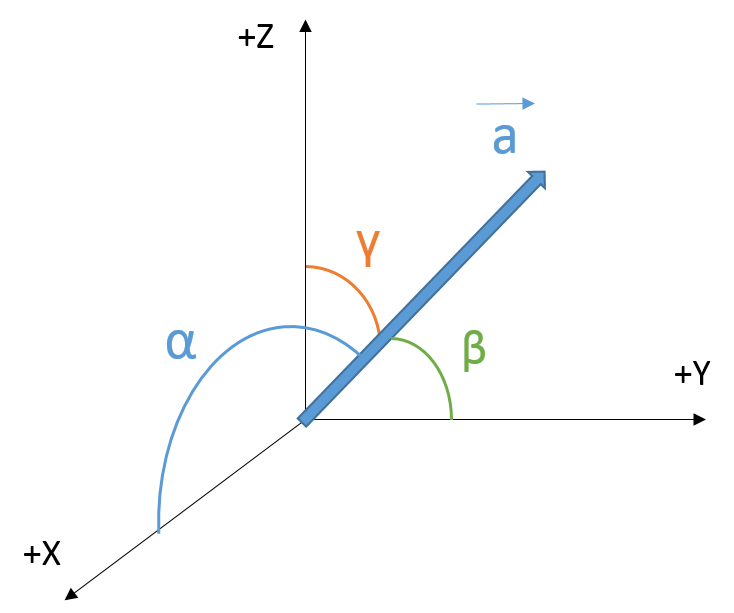
\includegraphics[width=10.5cm, height=8.0cm]{objs/cosenosDirectores.png}	
		\caption{Cosenos directores en el espacio.}
		\label{fig:cosenos_directores}
	\end{figure}
%**** imagen cosenos directores en el espacio\\

	La importancia de abordar este tópico se debe a que en desarrollo del presente trabajo se hace uso de los cosenos directores para determinar la dirección en que puntan los vectores resultado del análisis de componentes principales, por tanto se hace uso de esta característica geómetrica de los vectores para conecer el ángulo de orientación de los objetos.\\ 



\newpage
\thispagestyle{empty}
\mbox{}
\addtocounter{page}{-2}